\documentclass[border=12pt]{standalone}
\usepackage{tikz}
\usetikzlibrary{positioning, calc, fit, backgrounds, arrows.meta}
\usepackage{amsmath, amssymb}

\begin{document}
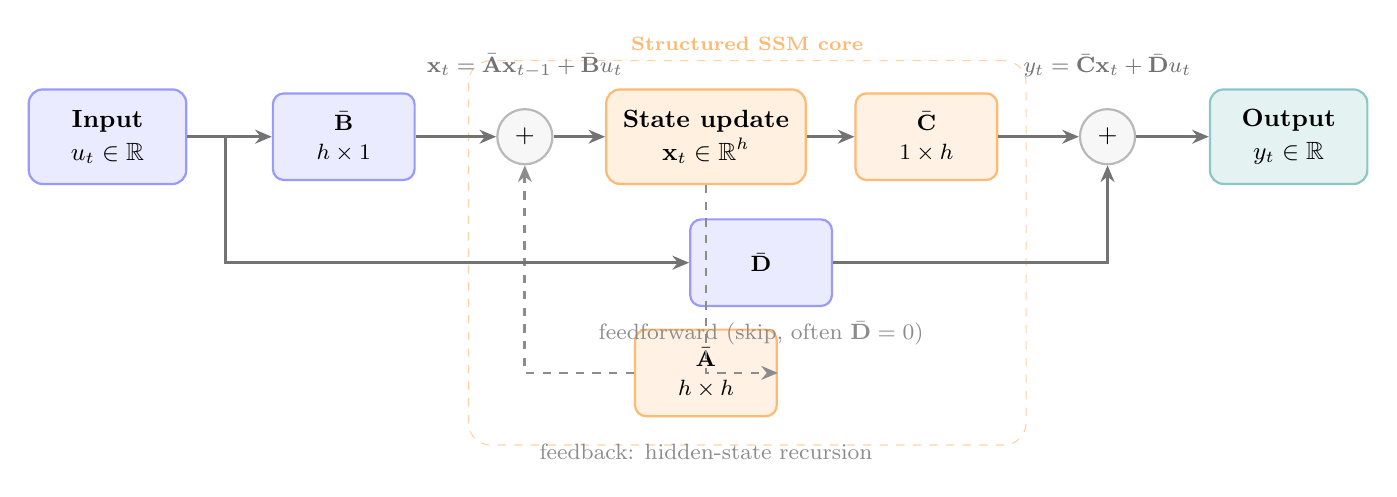
\begin{tikzpicture}[
    block/.style     = {rectangle, draw=gray!60, thick, rounded corners=5pt,
                        minimum height=1.4cm, minimum width=2.2cm,
                        font=\small, inner sep=6pt, align=center},
    smallblock/.style = {rectangle, draw=gray!55, thick, rounded corners=4pt,
                        minimum height=1.1cm, minimum width=1.8cm,
                        font=\footnotesize, inner sep=4pt, align=center},
    sig/.style       = {rectangle, draw=blue!40, thick, rounded corners=5pt,
                        fill=blue!8, minimum height=1.2cm, minimum width=2.0cm,
                        font=\small, inner sep=6pt, align=center},
    outsig/.style    = {rectangle, draw=teal!45, thick, rounded corners=5pt,
                        fill=teal!10, minimum height=1.2cm, minimum width=2.0cm,
                        font=\small, inner sep=6pt, align=center},
    state/.style     = {rectangle, draw=orange!55, thick, rounded corners=5pt,
                        fill=orange!12, minimum height=1.2cm, minimum width=2.0cm,
                        font=\small, inner sep=6pt, align=center},
    conn/.style      = {line width=1.0pt, draw=black!55,
                        -{Stealth[length=6pt, width=5pt]}},
    fbconn/.style    = {line width=1.0pt, draw=black!45, dashed,
                        -{Stealth[length=6pt, width=5pt]}},
    plus/.style      = {circle, draw=gray!55, thick, fill=gray!6,
                        minimum size=0.7cm, font=\small, inner sep=0pt},
    lbl/.style       = {font=\footnotesize, text=black!55, align=center},
]

%% ============================================================
%% LAYOUT (horizontal flow, left to right)
%% ============================================================

\node[sig]        (u)     at (0,   0)   {\textbf{Input}\\[1pt]$u_{t}\in\mathbb{R}$};
\node[smallblock, fill=blue!8, draw=blue!40]
                  (Bbar)  at (3.0, 0)   {\textbf{$\bar{\mathbf{B}}$}\\[1pt]\footnotesize $h\times 1$};
\node[plus]       (sum1)  at (5.3, 0)   {$+$};
\node[state]      (delay) at (7.6, 0)   {\textbf{State update}\\[1pt]$\mathbf{x}_{t}\in\mathbb{R}^{h}$};
\node[smallblock, fill=orange!10, draw=orange!55]
                  (Cbar)  at (10.4, 0)  {\textbf{$\bar{\mathbf{C}}$}\\[1pt]\footnotesize $1\times h$};
\node[plus]       (sum2)  at (12.7, 0)  {$+$};
\node[outsig]     (y)     at (15.0, 0)  {\textbf{Output}\\[1pt]$y_{t}\in\mathbb{R}$};

%% feedback block (Abar) below delay
\node[smallblock, fill=orange!10, draw=orange!55]
                  (Abar)  at (7.6, -3.0) {\textbf{$\bar{\mathbf{A}}$}\\[1pt]\footnotesize $h\times h$};

%% feedforward block (Dbar) below the main path
\node[smallblock, fill=blue!8, draw=blue!40]
                  (Dbar)  at (8.3, -1.6) {\textbf{$\bar{\mathbf{D}}$}};

%% ============================================================
%% CONNECTIONS
%% ============================================================

%% main forward path
\draw[conn] (u.east)     -- (Bbar.west);
\draw[conn] (Bbar.east)  -- (sum1.west);
\draw[conn] (sum1.east)  -- (delay.west);
\draw[conn] (delay.east) -- (Cbar.west);
\draw[conn] (Cbar.east)  -- (sum2.west);
\draw[conn] (sum2.east)  -- (y.west);

%% feedback x_t -> Abar -> sum1 (dashed)
\draw[fbconn] (delay.south) |- (Abar.east);
\draw[fbconn] (Abar.west) -| (sum1.south);

%% feedthrough u -> Dbar -> sum2
\coordinate (uTap) at (1.5, 0);
\draw[conn] (uTap) |- (Dbar.west);
\draw[conn] (Dbar.east) -| (sum2.south);

%% ============================================================
%% ANNOTATIONS
%% ============================================================

\node[lbl] at (5.3,  0.9)  {$\mathbf{x}_{t} = \bar{\mathbf{A}}\mathbf{x}_{t-1} + \bar{\mathbf{B}}u_{t}$};
\node[lbl] at (12.7, 0.9)  {$y_{t} = \bar{\mathbf{C}}\mathbf{x}_{t} + \bar{\mathbf{D}}u_{t}$};
\node[lbl, text=black!45] at (7.6, -4.0) {feedback: hidden-state recursion};
\node[lbl, text=black!45] at (8.3, -2.5) {feedforward (skip, often $\bar{\mathbf{D}}=0$)};

%% ============================================================
%% GROUPING BOX
%% ============================================================
\begin{scope}[on background layer]
    \node[draw=orange!35, dashed, rounded corners=8pt, inner sep=10pt,
          fit=(sum1)(delay)(Abar)(Cbar),
          label={[font=\scriptsize\bfseries, orange!55]above:%
                 Structured SSM core}] {};
\end{scope}

\end{tikzpicture}
\end{document}
